\documentclass[
BCOR2.0cm,							% Bindekorrektur, bspw. 1 cm
]
{scrbook}
\usepackage{ifpdf} 
\newif\ifpdf
\ifx\pdfoutput\undefined
	\pdffalse              	%normales LaTeX wird ausgef�hrt
\else
	\pdfoutput=1           
	\pdftrue               	%pdfLaTeX wird ausgef�hrt
\fi

\ifpdf
	%\usepackage{ae}        % Benutzen Sie nur
	%\usepackage{zefonts}  	% eines dieser Pakete
\else
	%%Normales LaTeX - keine speziellen Fontpackages notwendig
\fi

\ifpdf %%Einbindung von Grafiken mittels \includegraphics{datei}
	\usepackage[pdftex]{graphicx} %%Grafiken in pdfLaTeX
\else
	\usepackage[dvips]{graphicx} %%Grafiken und normales LaTeX
\fi


\ifpdf
	\pdfinfo
	{
    /Author (Andreas sterreicher)                                
    /Title (CMS)     
    /Subject (CMS - Handbuch)                                    
    /Keywords (CMS FH-Complete)
	}
\else			
\fi

\usepackage{listings} \lstset{numbers=left, numberstyle=\tiny, numbersep=5pt}
\lstset{language=tex} 


\usepackage[pdftex,colorlinks=true,urlcolor=blue,linkcolor=blue]{hyperref}
\usepackage[ngerman]{babel}		
\usepackage[T1]{fontenc}
\usepackage[latin9]{inputenc}
\usepackage{makeidx}
\usepackage{float}
\usepackage[small,bf]{caption}
\usepackage{fancyhdr}
\usepackage{amssymb,amsmath}
\usepackage{color}


\addtokomafont{chapter}{\color[rgb]{0.0,0.376,0.584}}
\addtokomafont{section}{\color[rgb]{0.0,0.376,0.584}}
\addtokomafont{subsection}{\color[rgb]{0.0,0.376,0.584}}


\renewcommand{\rmdefault}{phv} % Arial
\renewcommand{\sfdefault}{phv} % Arial

\makeindex

\graphicspath{{../../images/}}

\setlength{\tolerance}{2000}
\setlength{\parindent}{0pt}
\setlength{\parskip}{1ex plus 0.5ex minus 0.2ex}
\addtolength{\textheight}{2cm}
\addtolength{\headheight}{2pt}
\setlength{\captionmargin}{20pt}
\floatstyle{plain}
\floatname{example}{Example}

\newfloat{example}{hbtp}{loe}[chapter]
\floatplacement{figure}{hbtp}
\floatplacement{table}{htbp}

\newcommand{\dollar}{\char36}

\newenvironment{info}[1]{
    \hspace{-10mm}
    \fbox{
        \begin{minipage}{1cm}
        
\includegraphics[width=1cm]{icon_info}
        \end{minipage}
        \begin{minipage}{14.5cm}
        #1
        \end{minipage}
    }
}

\newenvironment{achtung}[1]{
    \hspace{-10mm}
    \fbox{
        \begin{minipage}{1cm}
        
\includegraphics[width=1cm]{icon_achtung}
        \end{minipage}
        \begin{minipage}{14.5cm}
        #1
        \end{minipage}
    }
}

\newenvironment{halt}[1]{
    \hspace{-10mm}
    \fbox{
        \begin{minipage}{1cm}
        
\includegraphics[width=1cm]{icon_halt}
        \end{minipage}
        \begin{minipage}{14.5cm}
        #1
        \end{minipage}
    }
}

\newenvironment{idee}[1]{
    \hspace{-10mm}
    \fbox{
        \begin{minipage}{1cm}
        
\includegraphics[width=1cm]{icon_idee}
        \end{minipage}
        \begin{minipage}{14.5cm}
        #1
        \end{minipage}
    }
}


\setlength{\unitlength}{1mm}

\newenvironment{markier}[5]{
    
    \thicklines \put(#2,#3){\vector(#4,#5){5}} \thinlines
    \put(#2,#3){\circle*{5}}
    \put(#2,#3){\textcolor{black}{\circle{5}}\makebox(-10,0){\textcolor{white}{#1}}}


}


\hyphenation{gleich-zeitig para-meter}


\begin{document}

\ifpdf
	\DeclareGraphicsExtensions{.pdf,.jpg,.png}
\else
	\DeclareGraphicsExtensions{.eps}
\fi

\pagestyle{fancyplain}
% Titelseite einbinden
%
% Titelseite, Abstrakt, Danksagung und Inhaltsverzeichnis
%
%% eigene Titelseitengestaltung %%%%%%%%%%%%%%%%%%%%%%%%%%%%%%%%%%%%%%%    

\begin{titlepage}
\begin{center}
\vspace*{40mm} \huge CMS-Handbuch\\
\vspace*{10mm}
\large \textsc{FH-Complete CMS}

\vfill 
\includegraphics[width=130mm]{fhcomplete}
	
\vfill \textsc{FH Technikum Wien}\\

Wien, \today
\end{center}
\end{titlepage}


\tableofcontents			% Inhaltsverzeichnis
\frontmatter					% Vorspann (z.B. roemische Seitenzahlen)
\chapter{Einleitung}
\mainmatter						% Hauptteil

%% Kapitel Anfang %%%%%%%%%%%%%%%%%%%%%%%%%%%%%%%%%%%%%%%%%%%%%%%%%

\chapter{Allgemeines}
\section{Ablauf}

\begin{figure}
	\centering
	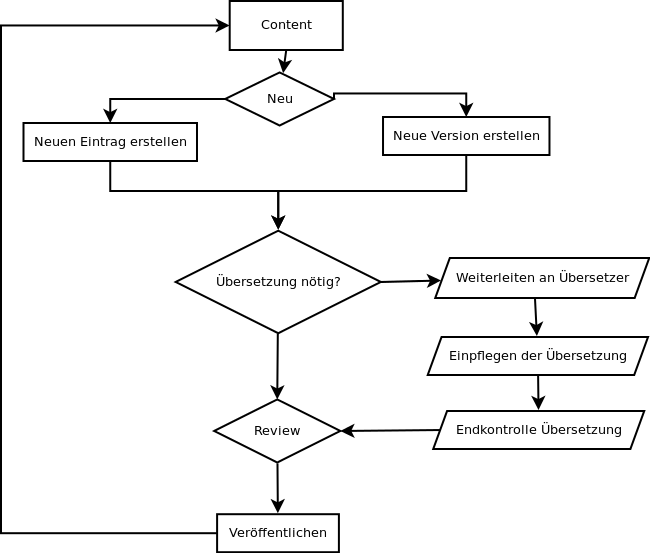
\includegraphics[width=0.75\textwidth]{CMS_Ablaufdiagramm.png}
	\caption{CMS Ablauf}
	\label{CMS Ablauf}
\end{figure}

\section{Men�aufbau}
Der Content kann in hierarchisch angeordnet werden. 
Dadurch ergibt sich die Men�struktur die im CIS verwendet wird.\\

\begin{figure}
	\centering
	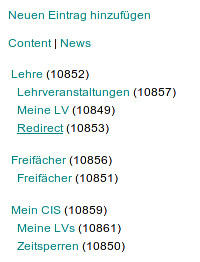
\includegraphics[width=0.30\textwidth]{CMS_Menue.png}
	\caption{CMS Men�struktur}
	\label{CMS Men�struktur}
\end{figure}

\section{Childs}
�ber den Punkt Childs k�nnen die Kindelemente eines Contents zugewiesen werden.
Dadurch wird die Men�struktur definiert. \\
Ein Content darf Child-Element von mehreren Contents sein. (mehrmals im Men�
vorkommen)\\
\\
\section{Zugriffsrechte}
�ber den Punkt Gruppen k�nnen Benutzergruppen zu Seiten zugeordnet werden. 
Nur Benutzer welche sich in diesen Gruppen befinden d�rfen die Seite betrachten.
Wenn keine Gruppe zugeordnet ist, ist die Seite f�r alle sichtbar.\\
Es k�nnen hier nur Gruppen ausgew�hlt werden, bei denen das Attribut Content 
auf true gesetzt ist.

\section{History}
Hier k�nnen die verschiedenen Versionen miteinander verglichen werden. 
Die Unterschiede zueinander werden farblich markiert. 
\chapter{Templates}
\section{Arten von Templates}
F�r den Content der Seiten stehen diverse Templates zur Verf�gung.
\subsection{Content mit Titel}
Dies ist das Standard-Template f�r normale Content Seiten. 
Es erstellt eine Seite mit �berschrift und statischem Content.
\subsection{Redirects}
Um auf Seiten zu verklinken, welche sich nicht im CMS befinden, 
ist das Redirect Template zu verwenden. Hier kann auf eine beliebige URL 
verlinkt werden.\\
In der Redirect URL k�nnen Variablen verwendet werden.\\
z.B.: news.php?stg\_kz=\$stg\_kz
\\
\subsection{Includes (Addons)}
Das Men� besteht teilweise aus dynamischem Content. Dieser kann �ber 
Includes (Addons) erzeugt werden. Bei diesem Template wird die URL zu einem PHP
Script angegeben welches sich im Verzeichnis /cms/menu/ befindet.\\ 
Dieses Script enth�lt eine Klasse welche von der menu\_addon Klasse abgeleitet
ist. Die Klasse erzeugt den Content der unterhalb des Men�punkts angezeigt wird.
\\
\subsection{News}
Neue News werden generell nicht �ber das CMS-System angelegt.\\ 
Zum Anlegen von neuen News-Eintr�gen ist die Newsverwaltung zu verwenden.\\
Nach dem Anlegen eines Newseintrages k�nnen die sprachspezifischen Daten 
�ber das CMS System verwaltet werden. Dazu kann im oberen Teil des Men�s 
auf den Reiter News gewechselt werden. Hier werden die neuesten Newseintr�ge 
angezeigt und k�nnen editiert werden.\\

\section{Anwendungsf�lle}
Im folgenden werden diverse Beispiele f�r die Verwendung von Templates
aufgezeigt.

\subsection{Link auf eigenen Men�baum}
Im Men� k�nnen Links eingef�gt werden, welche auf ein Untermen� verweisen.
Es wird dann nur das angegebene Submen� angezeigt. (zb Freif�cher, Lehre,
Mein CIS):\\
\\
	template: 	Redirect\\
	url: 		?content\_id=12\\
	target: 	\_self\\
\\
Wenn das angezeigt Men� nicht das Start Men� ist, wird automatisch ein Zur�ck
Button anzeigt.\\
\subsection{Link auf PHP Scripte}
Links auf PHP-Seiten k�nnen mit dem Redirect Template eingef�gt werden:\\
\\
	template: 	Redirect\\
	url:		../cis/private/script.php\\
	target:		content\\
\\
\subsection{Anlegen eines Links auf einen anderen Content}
Ein Content kann an mehreren Stellen im Men�baum eingeh�ngt werden.
Sollen die Men�eintr�ge jedoch unterschiedlich benannt werden, muss einer
der Eintr�ge als Redirect auf den anderen angelegt werden.\\ 
\\
	template: 	Redirect\\
	url:		../cms/content.php?content\_id=12\\
	target:		content\\
\\
\subsection{Include Men� Addons}
Anlegen eines Include Men� Addons 
(zB LV-Auswahl, Freif�cherliste, MeineLVs, Zeitsperren, etc)\\
\\
	template: 	include\\
	url:		menu\_addon\_meinelv.inc.php\\
\\
\subsection{Abstand im Men�baum}
Wenn zwischen den Men�eintr�gen ein Abstand eingef�gt werden soll, muss dies
�ber das Spacer-Addon geschehen.\\
\\
	template:	include\\
	url:		menu\_addon\_spacer.inc.php\\
\\
Diese Seite kann dann als Child zum Men� hinzugef�gt und an der entsprechenden
Stelle plaziert werden. Dadurch entsteht eine Leerzeile
	
\subsection{Links mit Variablen}
Bei manchen Links m�ssen Variablen als Parameter �bergeben werden (zB
Newsverwaltung)\\
Diese k�nnen bei Redirects mittels \$variablenname eingef�gt werden.\\
\\
	template: 	redirect\\
	url:	
	../cms/newsverwaltung.php?studiengang\_kz=\$studiengang\_kz\&semester=\$semester\\
\\
Die Variablen werden entweder durch ein IncludeAddon gesetzt, oder als Parameter 
an das menue.php uebergeben.\\
\\
\subsection{Men�eintrag zum Aufklappen ohne Link}
Men�eintr�ge die nur zur Gruppierung der Links verwendet werden, und selbst
keinen Content haben k�nnen mittels Redirect Template angelegt werden.
Dadurch bleibt die derzeit angezeigte Seite bestehen und es wird nur das
Men� auf und zu geklappt. (zB Lehre)\\
\\
	template: 	Redirect\\
	url:		\#Lehre\\
	target:		\_self\\
\\

\chapter{Versionierung}
Der Content einer Seite kann Versioniert werden. 
�ber den Punkt "neue Version anlegen" kann eine neue Version erstellt werden.
Diese kopiert die bestehende Version und setzt diese auf nicht sichtbar.\\ 
Diese Version kann nun bearbeitet werden. 
Im CIS wird nach wie vor die alte Version angezeigt. 
Erst wenn das sichtbar Attribut gesetzt wird (bzw nach Review), scheint die neue
Version im CIS auf. Im CIS wird immer nur die neueste sichtbare Version
angezeigt.\\
\\
Zur �bersicht ist darauf zu achten, dass die Versionen der verschiedenen Sprachen 
gleichl�ufig sind. (d.h. Version 2 in Deutsch sollte den entsprechenden Inhalt auch in Version 2 in Englisch enthalten)

\chapter{�bersetzungen}
Ein Content kann in beliebig viele Sprachen �bersetzt werden.\\
Wenn keine �bersetzung in der Anzeigesprache vorhanden ist, wird automatisch die
DEFAULT\_LANGUAGE angezeigt.\\
�ber den Button "�bersetzer benachrichtigen" wird
ein automatisches Mail an den eingetragenen �bersetzer gesendet, 
damit dieser den Content �bersetzt. \\
Pro Organisationseinheit k�nnen unterschiedliche �bersetzer eingetragen
werden.\\
Wird f�r die aktuelle Organisationseinheit kein �bersetzer gefunden, 
wird automatisch der dar�berliegende �bersetzer verst�ndigt. 
Wenn im Tree �berhalb keiner gefunden wird, werden alle �bersetzer
benachrichtigt. \\
�bersetzer k�nnen im FAS �ber den Karteireiter Funktionen
zugeteilt werden. (Funktion: translate)

\chapter{Review}
�ber den Button ''Review anfordern'' kann ein Review-Team benachrichtigt werden. 
Diese k�nnen den Content pr�fen und danach best�tigen. \\
Dazu wird ein eigener Button angezeigt, sofern die Berechtigung dazu vorhanden
ist. Beim Best�tigen des Contents (Review OK / Publish) wird dieser automatisch
auf sichtbar gesetzt.\\
\\ 
Pro Organisationseinheit k�nnen unterschiedliche Reviewer eingetragen werden. 
Wird f�r die aktuelle Organisationseinheit kein Reviewer gefunden, 
wird automatisch der dar�berliegende Reviewer verst�ndigt. 
Wenn im Tree �berhalb keiner gefunden wird, werden alle Reviewer benachrichtigt.\\
Der Reviewer kann im FAS �ber den Karteireiter Funktionen zugeteilt werden.
(Funktion: review)

\chapter{Dokumentenmanagement}
Das CMS System ist mit einem Dokumentenmanagementsystem gekoppelt. 
Klickt man auf das Symbol zum Einf�gen eines Links oder eines Bildes 
erh�lt man neben dem Eingabefeld f�r die URL ein kleines Symbol (1).
\begin{figure}
	\begin{center}
    \begin{picture}(56,45)
			\put(0,0){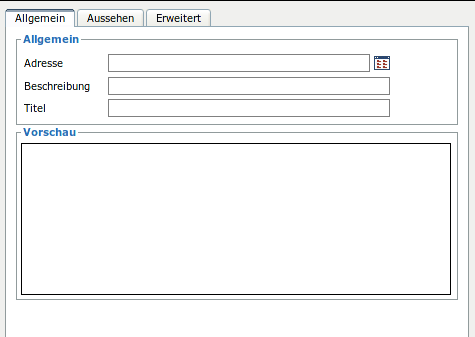
\includegraphics[height=40mm, width=56mm]{dms_erweitert_icon.png}}
			\markier{1}{52}{39}{-1}{-1}
		\end{picture}
    \caption{Dokumentenauswahl}
		\label{Dokumentenauswahl}
  \end{center}
\end{figure}

Hier gelangt man in das Dokumentenmanagementsystem.
Dokumente k�nnen hier hochgeladen und Kategorien zugeordnet werden. 
Mit einem klick auf den Namen wird die Datei ausgew�hlt und in den Editor eingef�gt.
\section{Hochladen von Dateien}
- Kategorie ausw�hlen\\
- "Datei hochladen" klicken\\
- im unteren Teil wird ein Formular angezeigt. Hier kann die Datei gesucht und
hochgeladen werden. \\
\section{Neue Version hochladen}
- Datei suchen\\
- Erweitert->Neue Version hochladen\\
- Datei ausw�hlen und hochladen\\

\section{Kategorien}
Damit die Dokumente nicht bunt durcheinandergemisch sind, k�nnen diese in
Kategorien zusammengefasst werden. Ein Dokument kann immer nur einer Kategorie
zugewiesen sein.

\section{Zugriffsrechte}
Der Zugriff auf Dokumente wird �ber die Kategorien gesteuert.\\
Zu jeder Kategorie k�nnen Gruppen zugeordnet werden. Die Mitglieder dieser Gruppe haben
dann Zugriff auf die Dokumente innerhalb dieser Kategorie. Die Rechte werden an die
darunterliegenden Kategorien vererbt.\\
Wenn keine Gruppenzuordnung f�r die Kategorie oder �bergeordneten Kategorien vorhanden ist, dann ist die Datei frei f�r alle zug�nglich.\\
\\
Eine Ausnahme stellen die Projektdokumente dar. Sobald ein Dokument zu einem Projekt zugeordnet ist, ist dieses Dokument nur noch von den Personen einsehbar, welche dem entsprechenden Projekt zugeordnet sind.\\
\\
F�r Administratoren kann die Berechtigung 'basis/dms' vergeben werden. Mit diesem Recht kann auf alle Dokumente zugegriffen werden.\\
\\
Gesperrte Kategorien werden im DMS System mit einem Schloss Symbol versehen.
\chapter{Administratives}
\section{DMS}
Die Dateien werden im DMS\_PATH abgelegt. Die Berechtigung wird f�r die Gruppe
"dms" gesetzt! Diese Gruppe muss am Server vorhanden sein, da es sonst 
m�glicherweise zu problemen beim Zugriff kommt.\\
\section{Import}
Ist die Datei gr��er als 15 MB (PHP upload\_max\_filesize) kann sie �ber den
Import Ordner hochgeladen werden. Die Datei wird vorher per WinSCP etc in den
Import Ordner (siehe Config) kopiert. Die Dateien des Import Ordners werden unterhalb des Formulars angezeigt und 
k�nnen mittels ''Hochladen'' ins DMS �bernommen werden
\section{Men� Addons}
Include Addons befinden sich unter /cms/menu/. Pro Addon gibt es ein eigenes
File. Darin befindet sich eine Klasse die von der Klasse menu\_addon abgeleitet
ist. Diese Klasse bef�llt Variablen der Basisklasse welche dann ausgegeben werden.
\section{Startpunkt des CMS}
Der Content bei dem das Men� im CIS beginnt kann �ber eine Config Variable
definiert werden.


%% Kapitel Ende   %%%%%%%%%%%%%%%%%%%%%%%%%%%%%%%%%%%%%%%%%%%%%%%%%
\appendix							% Beginn des Anhangs
\chapter{Schluss}
\listoftables					% Tabellenverzeichnis
\listoffigures				% Abbildungsverzeichnis
\end{document}
